\documentclass[11pt]{article}
\usepackage[margin=1in]{geometry}
\usepackage{amsmath,amssymb,amsthm}
\usepackage{booktabs,array,tabularx}
\usepackage{graphicx}
\usepackage{enumitem}
\usepackage{float}
\usepackage[hidelinks]{hyperref}
\graphicspath{{figures/}{../figures/}}
\emergencystretch=3em
\setlength{\parindent}{0pt}
\setlength{\parskip}{6pt}
\renewcommand{\arraystretch}{1.2}

% ---------- macros ----------
\newcommand{\R}{\mathbb{R}}
\renewcommand{\Pr}{\mathbb{P}}
\newcommand{\Cov}{\operatorname{Cov}}
\newcommand{\one}{\mathbf{1}}
\newcommand{\T}{^{\top}}
\newcommand{\hSigma}{\hat{\Sigma}}
\newcommand{\hmu}{\hat{\mu}}
\newcommand{\norm}[1]{\lVert #1\rVert}
\newcommand{\code}[1]{\texttt{#1}}

\theoremstyle{plain}
\newtheorem{proposition}{Proposition}
\setcounter{proposition}{1}

\title{\textbf{Keystroke Anomaly Detection with the Mahalanobis Distance}\\[4pt]
\large DS5020 Final Project, Iteration 3: Worked Example, Implementation and Verification}
\author{Nikhil Chaganti \and Trung Pham}
\date{Fall 2026}

\begin{document}
\maketitle
\tableofcontents

% =====================================================================
\section{Overview}
In this iteration we turn the Iteration 2 math into code and check it three ways:
a tiny example computed exactly, a simulation where the truth is known, and the
real keystroke data compared with library results. All code is in \code{src/}:

\begin{itemize}[nosep]
\item \code{methods.py}: one function per algorithm step, NumPy only.
\item \code{simulate.py}: the Iteration 2 simulation as functions.
\item \code{small\_example.py}, \code{check\_simulation.py}, \code{run\_real.py}:
  the three tests. Every number in this report is printed by one of them.
\end{itemize}

Theorem and assumption numbers (Theorems 1 to 5, Proposition 1, A1 to A6) refer to the
Iteration 2 report.

\textbf{What stayed the same.} The dataset (CMU Keystroke Benchmark), the 21
features H and UD, the simulation model ($p=5$, $\mu=0$, $\Sigma=BB\T+5I$),
$n=5000$, $\alpha=0.01$ and the seed \code{np.random.default\_rng(0)}. The code
reproduces the Iteration 2 estimates exactly (for example $\hmu_1=0.0529$).

\textbf{What changed, and why.}
\begin{enumerate}[nosep]
\item Steps 4 to 6 now use the Cholesky factor $L$ of $\hSigma$ instead of the
  eigendecomposition. Cholesky can be written from scratch in a few lines, it fails
  exactly when $\hSigma$ is not positive definite (a built-in check of A3), and it
  gives the same $d^2$ (Proposition~\ref{prop:chol}).
\item The threshold $\tau$ is now computed from scratch (Step 7) instead of with
  SciPy, which is used only to check it.
\item The heavy-tailed stress test uses its own random stream, so its single-run
  false-alarm rate is $0.053$ instead of the Iteration 2 value $0.057$. The averages
  over 200 runs agree ($0.0529$ now, $0.0526$ before).
\end{enumerate}

% =====================================================================
\section{New Notation}
\begin{table}[H]
\centering\small
\begin{tabular}{@{}l p{9.2cm} l@{}}
\toprule
Symbol & Meaning & Dimension\\
\midrule
$L$ & lower-triangular Cholesky factor, $\hSigma=LL\T$, with $L_{jj}>0$ & $\R^{p\times p}$\\
$z$ & $z=L^{-1}(x-\hmu)$, found by forward substitution & $\R^{p}$\\
$r$ & repetition index of an attempt, $r=50(\text{session}-1)+\text{rep}$ & $1,\dots,400$\\
$\kappa(\hSigma)$ & condition number $\lambda_{\max}/\lambda_{\min}$ & scalar\\
$\varepsilon$ & ridge added to the diagonal, $\hSigma+\varepsilon I$ & scalar $>0$\\
$g_1$, $g_2$ & sample skewness and excess kurtosis of one feature & scalars\\
$\rho_1$ & lag-1 autocorrelation of a sequence & scalar\\
\bottomrule
\end{tabular}
\end{table}
All other symbols are as in the Iteration 2 notation table.

% =====================================================================
\section{The Algorithm (Updated)}\label{sec:algo}

\begin{proposition}\label{prop:chol}
Let $\Sigma$ be positive definite with Cholesky factor $L$ ($\Sigma=LL\T$, $L$ lower
triangular with positive diagonal). Then $\Sigma^{-1}=L^{-\top}L^{-1}$,
$d^2(x)=\norm{L^{-1}(x-\mu)}^2$, and if $x\sim\mathcal N(\mu,\Sigma)$ then
$\Cov(L^{-1}(x-\mu))=I$.
\end{proposition}
\begin{proof}
$L$ is invertible because its diagonal is positive [determinant of a triangular
matrix is the product of the diagonal]. Then
$(LL\T)^{-1}=L^{-\top}L^{-1}$ [$(AB)^{-1}=B^{-1}A^{-1}$], so
$d^2=(x-\mu)\T L^{-\top}L^{-1}(x-\mu)=\norm{L^{-1}(x-\mu)}^2$. Finally
$\Cov(L^{-1}(x-\mu))=L^{-1}\Sigma L^{-\top}=L^{-1}LL\T L^{-\top}=I$. So $z=L^{-1}(x-\mu)$
whitens the data just like $\Sigma^{-1/2}(x-\mu)$ in Theorem~4, and the proof of
Theorem~3 ($d^2\sim\chi^2_p$) holds unchanged with this $z$.
\end{proof}

\textbf{Cholesky formulas.} Equating entries of $\hSigma=LL\T$ column by column gives
\[
L_{jj}=\Big(\hSigma_{jj}-\sum_{k<j}L_{jk}^2\Big)^{1/2},\qquad
L_{ij}=\frac{1}{L_{jj}}\Big(\hSigma_{ij}-\sum_{k<j}L_{ik}L_{jk}\Big)\quad(i>j).
\]
If the number under the square root is $\le0$, then $\hSigma$ is not positive definite
and the function stops.

\textbf{Chi-squared quantile.} $F_p(x)=P(\tfrac p2,\tfrac x2)$ with
$P(s,y)=y^se^{-y}\sum_{k\ge0}y^k/\Gamma(s+k+1)$ (series for the regularized incomplete
gamma function, with $\Gamma$ of half-integers from $\Gamma(\tfrac12)=\sqrt\pi$ and
$\Gamma(s+1)=s\Gamma(s)$). Since $F_p$ is continuous and increasing, $\tau$ is found by
bisection on $F_p(\tau)=1-\alpha$.

\begin{table}[H]
\centering\small
\begin{tabularx}{\linewidth}{@{}c>{\raggedright\arraybackslash}X>{\raggedright\arraybackslash}p{3.6cm}>{\raggedright\arraybackslash}p{2.6cm}@{}}
\toprule
Step & Equation & Function in \code{methods.py} & Operations\\
\midrule
1 & $\hmu=\frac1nX\T\one$ & \code{my\_mean} & $np$\\
2 & $X_c=X-\one\hmu\T$ & \code{my\_center} & $np$\\
3 & $\hSigma=\frac1nX_c\T X_c$ & \code{my\_covariance} & $np^2$\\
4 & $\hSigma=LL\T$ (formulas above; stops if not PD) & \code{my\_cholesky} & $p^3/3$\\
5 & solve $Lz_j=y_j-\hmu$ by forward substitution & \code{my\_forward\_sub} & $p^2$ per attempt\\
6 & $\hat d_j^2=z_j\T z_j$ & \code{my\_mahalanobis2} & $p$ per attempt\\
7 & $\tau=F_p^{-1}(1-\alpha)$ by bisection & \code{my\_threshold} & a few thousand\\
8 & flag attempt $j$ if $\hat d_j^2>\tau$ & \code{my\_flag} & 1 per attempt\\
9 & rate $=$ (number flagged) / (number of attempts) & \code{my\_rate} & $m$\\
\midrule
Q2 & $[\hSigma\mid I]\to[I\mid\hSigma^{-1}]$ by Gauss-Jordan; also $\hSigma^{-1}=L^{-\top}L^{-1}$ & \code{my\_inverse}, \code{my\_cholesky\_inverse} & $p^3$\\
A3 & $\kappa=\lambda_{\max}/\lambda_{\min}$ by power and inverse iteration & \code{my\_condition\_number} & $p^2$ per iteration\\
\bottomrule
\end{tabularx}
\end{table}

% =====================================================================
\section{Iteration 3 -- Math Questions}\label{sec:questions}

\subsection{Question 1: the small worked example}
\textbf{Data.} $n=4$ attempts with $p=2$ features, and one new attempt:
\[
X=\begin{pmatrix}0&0\\2&1\\2&3\\4&4\end{pmatrix},\qquad x=\begin{pmatrix}4\\3\end{pmatrix}.
\]
All values below are exact fractions printed by \code{src/small\_example.py}.

\textbf{Step 1, mean (Theorem 1).} $X\T\one=(8,8)\T$, so $\hmu=\frac14(8,8)\T=(2,2)\T$.

\textbf{Step 2, centring.} Subtract $\hmu$ from every row:
$X_c=\begin{pmatrix}-2&-2\\0&-1\\0&1\\2&2\end{pmatrix}$.

\textbf{Step 3, covariance (Theorem 1, divisor $n$).}
\[
X_c\T X_c=\begin{pmatrix}8&8\\8&10\end{pmatrix},\qquad
\hSigma=\frac14X_c\T X_c=\begin{pmatrix}2&2\\2&5/2\end{pmatrix},\qquad
\det\hSigma=2\cdot\tfrac52-2\cdot2=1.
\]
Since $\hSigma_{11}>0$ and $\det\hSigma>0$, $\hSigma$ is positive definite (A3 holds).

\textbf{Inverse by Gauss-Jordan (Question 2).} Row operations on $[\hSigma\mid I]$:
\[
\left[\begin{array}{cc|cc}2&2&1&0\\2&\tfrac52&0&1\end{array}\right]
\xrightarrow{R_1/2}
\left[\begin{array}{cc|cc}1&1&\tfrac12&0\\2&\tfrac52&0&1\end{array}\right]
\xrightarrow{R_2-2R_1}
\left[\begin{array}{cc|cc}1&1&\tfrac12&0\\0&\tfrac12&-1&1\end{array}\right]
\xrightarrow{2R_2}
\left[\begin{array}{cc|cc}1&1&\tfrac12&0\\0&1&-2&2\end{array}\right]
\xrightarrow{R_1-R_2}
\left[\begin{array}{cc|cc}1&0&\tfrac52&-2\\0&1&-2&2\end{array}\right],
\]
so $\hSigma^{-1}=\begin{pmatrix}5/2&-2\\-2&2\end{pmatrix}$.

\textbf{Mahalanobis distance (Theorem 2).} $x-\hmu=(2,1)\T$,
$\hSigma^{-1}(x-\hmu)=(3,-2)\T$, and
\[
d^2(x)=(2,1)\begin{pmatrix}3\\-2\end{pmatrix}=6-2=4.
\]

\textbf{Decision (Theorem 5).} For $p=2$ the $\chi^2_2$ CDF is $1-e^{-x/2}$, so
$\tau=-2\log\alpha$: $\tau=5.991$ at $\alpha=0.05$ and $9.210$ at $\alpha=0.01$. Since
$d^2=4<\tau$, the new attempt is not flagged at either level.

\textbf{Second-way checks.}
\begin{itemize}[nosep]
\item $\hSigma\hSigma^{-1}=I$ exactly, in fractions.
\item The Cholesky route (Steps 4 to 6) in floating point:
  $L=\begin{pmatrix}\sqrt2&0\\\sqrt2&1/\sqrt2\end{pmatrix}$, since $L_{11}=\sqrt2$,
  $L_{21}=2/\sqrt2$ and $L_{22}=\sqrt{5/2-2}$. Forward substitution gives
  $z=L^{-1}(x-\hmu)=(\sqrt2,-\sqrt2)\T$ and $z\T z=4$, equal to the exact value up to
  $4\times10^{-15}$ (Proposition~\ref{prop:chol}).
\item Our bisection threshold matches $-2\log\alpha$ to $1.3\times10^{-13}$.
\end{itemize}

\subsection{Question 2: inverse and Cholesky from scratch}
\code{my\_inverse} is Gauss-Jordan elimination with partial pivoting (it also runs
on exact fractions, as above). \code{my\_cholesky} uses the formulas in
Section~\ref{sec:algo}, and \code{my\_cholesky\_inverse} computes
$L^{-\top}L^{-1}$ with forward substitution. Compared with
\code{numpy.linalg.inv} and \code{numpy.linalg.cholesky}:

\begin{table}[H]
\centering\small
\begin{tabular}{@{}llrr@{}}
\toprule
Data & Quantity & max $|$mine $-$ numpy$|$ & relative error\\
\midrule
Simulation ($p=5$) & $\hSigma^{-1}$ (Gauss-Jordan) & $2.8\times10^{-17}$ & $9.3\times10^{-17}$\\
Simulation ($p=5$) & $\hSigma^{-1}$ (Cholesky) & $5.6\times10^{-17}$ & $2.0\times10^{-16}$\\
Simulation ($p=5$) & $L$ & $8.7\times10^{-19}$ & $1.3\times10^{-19}$\\
Real data, log H ($p=21$) & $\hSigma^{-1}$ (Gauss-Jordan) & $6.8\times10^{-13}$ & $5.1\times10^{-16}$\\
Real data, log H ($p=21$) & $\hSigma^{-1}$ (Cholesky) & $4.6\times10^{-13}$ & $3.6\times10^{-16}$\\
Real data, log H ($p=21$) & $L$ & $2.8\times10^{-17}$ & $7.3\times10^{-17}$\\
\bottomrule
\end{tabular}
\end{table}
All relative errors are at the level of double-precision rounding ($\approx10^{-16}$).
The absolute differences on the real data are larger only because the entries of
$\hSigma^{-1}$ are large (the timings are small numbers in seconds). The two methods
do the same arithmetic in a different order, so they differ by rounding only.

\subsection{Question 3: QQ plot of $d^2$ against $\chi^2_{21}$}
Figure~\ref{fig:realqq} plots the sample quantiles of $\hat d^2$ for subject s002
against the quantiles of $\chi^2_{21}$ (our own \code{my\_chi2\_quantile}).

\begin{figure}[H]
\centering
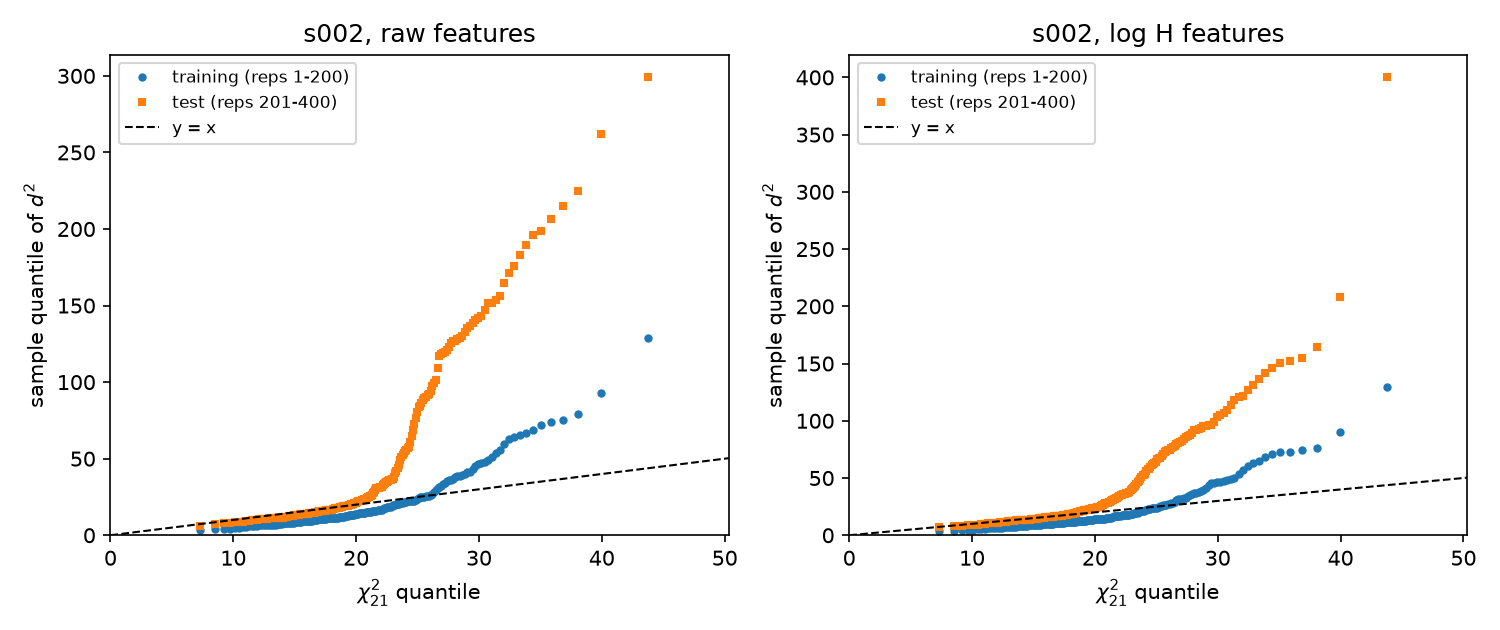
\includegraphics[width=\linewidth]{it3_real_qq.png}
\caption{QQ plots of $\hat d^2$ against $\chi^2_{21}$ for s002, raw features (left) and
log hold times (right). If the model were right, the points would lie on the line
$y=x$.}\label{fig:realqq}
\end{figure}

\textbf{The fit is not good.} In the middle the training points lie below the line
(median $14.0$ against $20.3$ for $\chi^2_{21}$, with log hold times), which is
expected because the same data were used to fit $\hmu$ and $\hSigma$. The upper tail
is far too heavy: the 99th percentile of $\hat d^2$ on the test attempts is $173$
against $38.9$ for $\chi^2_{21}$. The Kolmogorov-Smirnov $p$-values are below
$10^{-21}$. For comparison, the same plot on simulated normal data lies on the line
(Figure~\ref{fig:simqq}).

\subsection{Question 4: normality of each feature}
We computed the skewness $g_1$ and excess kurtosis $g_2$ of each feature on the 200
training attempts of s002 (for normal data both are about $0$, and 3 standard errors
are $0.52$ and $1.04$).

\begin{figure}[H]
\centering
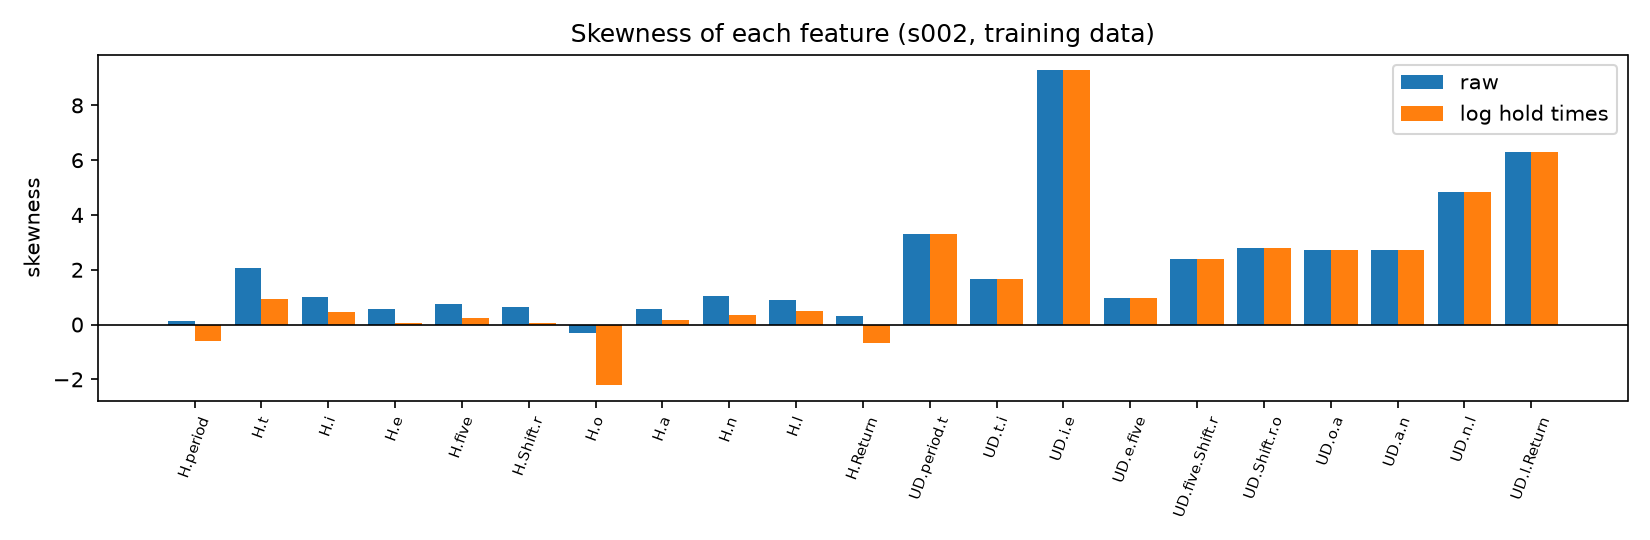
\includegraphics[width=\linewidth]{it3_real_skewness.png}
\caption{Skewness of each feature, raw and with log hold times (UD features cannot be
logged, so their two bars are equal).}\label{fig:skew}
\end{figure}

\begin{figure}[H]
\centering
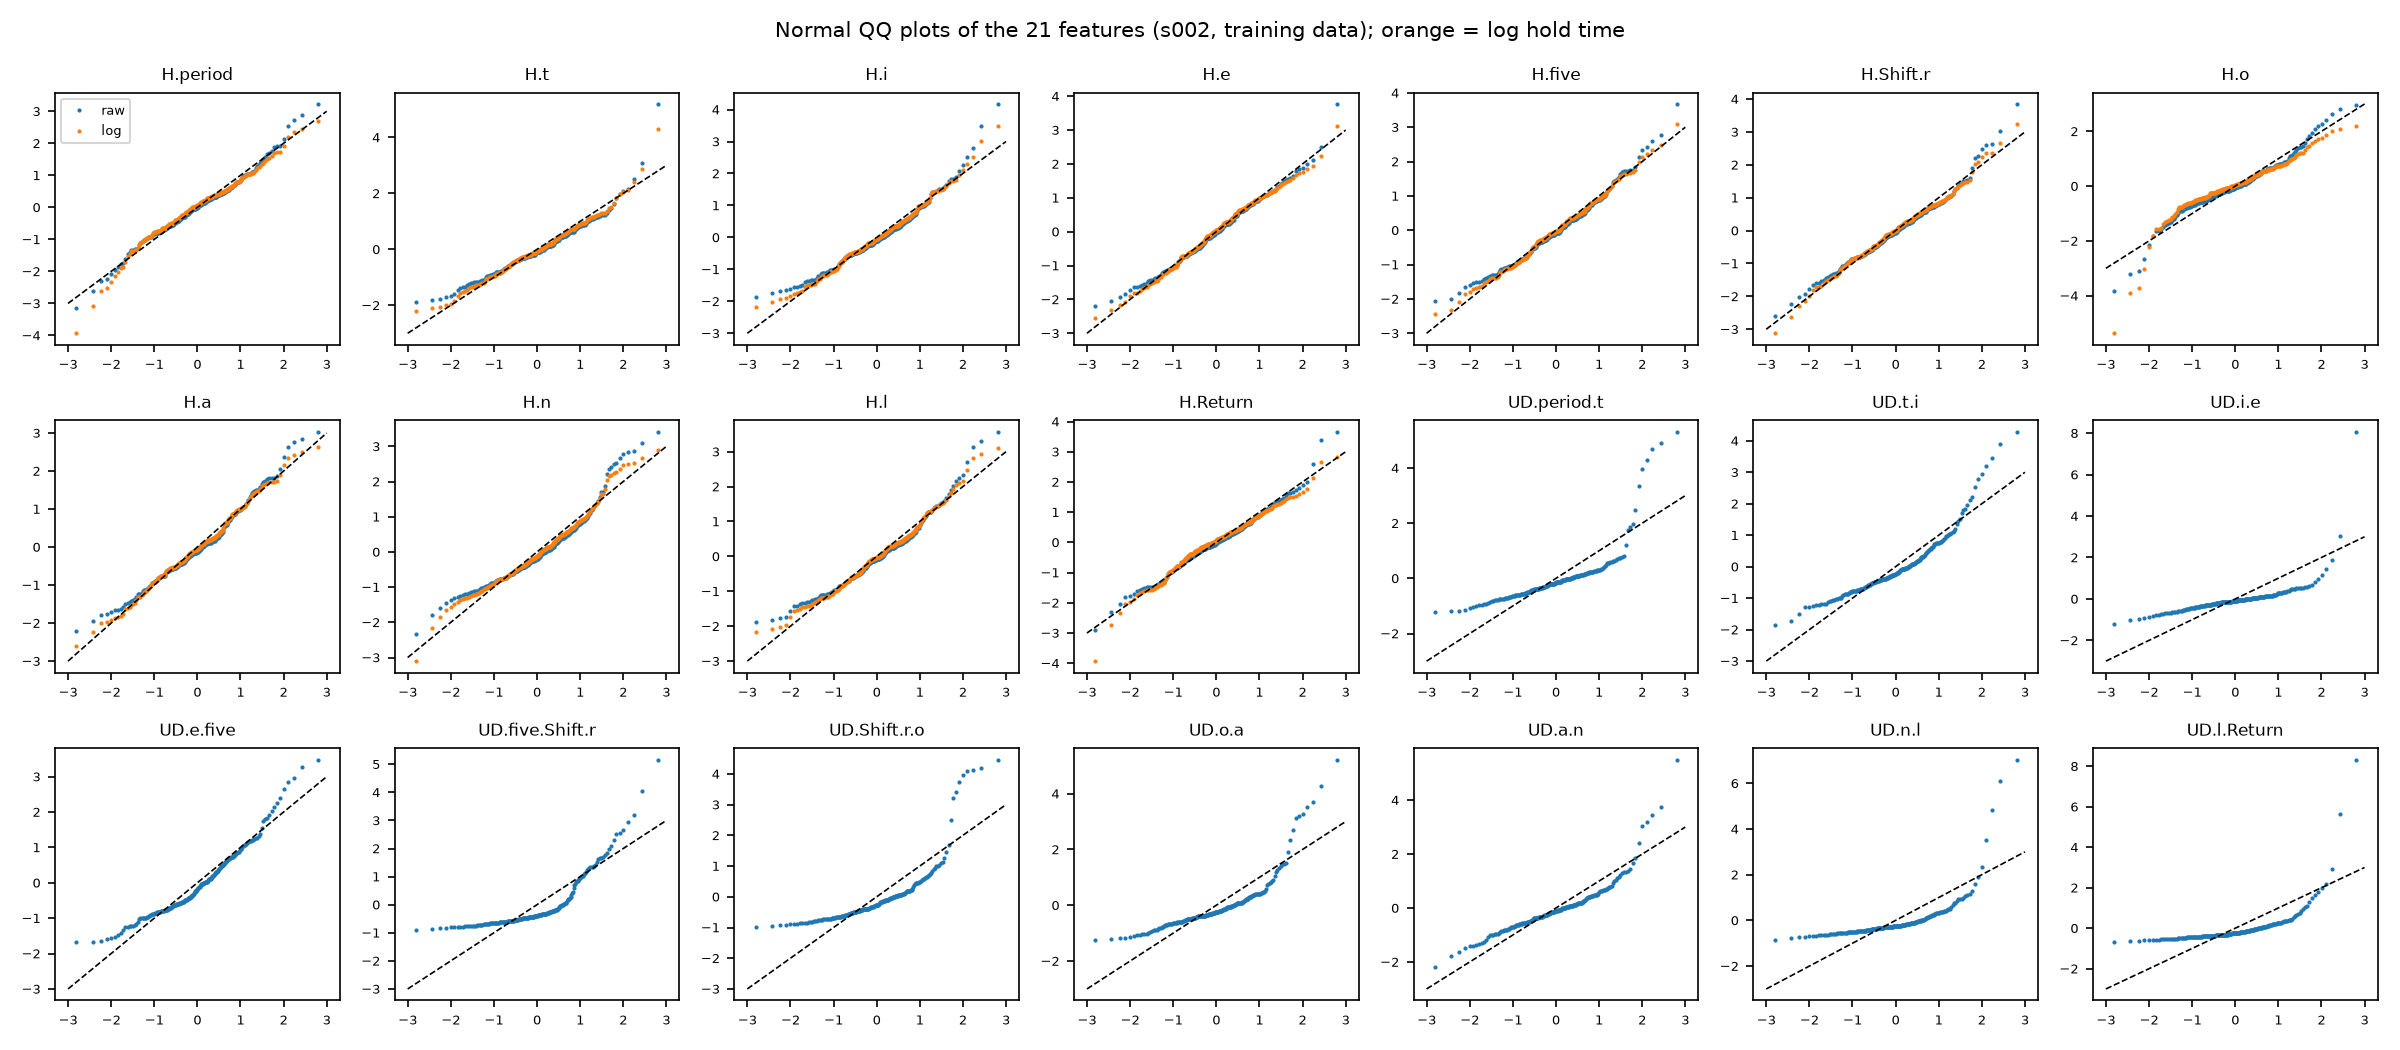
\includegraphics[width=\linewidth]{it3_real_feature_qq.png}
\caption{Normal QQ plots of the 21 standardized features of s002. Blue: raw. Orange:
log hold time.}\label{fig:featqq}
\end{figure}

\textbf{Features that break normality} (rule: $|g_1|>1$ or $|g_2|>3$):
\begin{itemize}[nosep]
\item \textbf{All 10 UD features.} They are strongly right-skewed with heavy tails
  ($g_1$ from $0.98$ to $9.28$, $g_2$ up to $107$ for \code{UD.i.e}). A few long
  pauses between keys create the tail. They cannot be log-transformed because some
  values are negative.
\item \textbf{Hold times, raw:} \code{H.t}, \code{H.i} and \code{H.n}. The log
  transform lowers the median $|g_1|$ of the hold times from $0.65$ to $0.46$ and fixes
  \code{H.i} and \code{H.n}, but \code{H.t} stays skewed and \code{H.o} becomes
  left-skewed ($g_1=-2.20$) because of a few very short holds.
\end{itemize}
So 12 of 21 features fail with raw data and 11 of 21 with log hold times. The UD
features are the main reason the $\chi^2$ threshold is badly calibrated.

\subsection{Question 5: a singular or nearly singular $\hSigma$}
\textbf{Exactly singular.} With all 31 features, \code{my\_cholesky} stops at pivot 3
(value $6.9\times10^{-18}$) because $\text{DD}=\text{H}+\text{UD}$ makes $\hSigma$ singular
(rank 21 of 31, \code{numpy.linalg.cond} $=9.6\times10^{17}$). The right fix is to remove
the dependent columns, which is why we keep only H and UD.

\textbf{Nearly singular.} With the 21 features $\hSigma$ is positive definite, and its
condition number is $\kappa=1602$ for raw data and $134$ with log hold times. A large
$\kappa$ means a small error in $\hSigma$ can cause a large error in $\hSigma^{-1}$ and so
in $\hat d^2$. If $\kappa$ were too large, we would add a ridge, $\hSigma+\varepsilon I$,
which raises every eigenvalue by $\varepsilon$ and lowers $\kappa$:

\begin{table}[H]
\centering\small
\begin{tabular}{@{}lrrr@{}}
\toprule
Ridge $\varepsilon$ (log H data) & $\kappa$ & false-alarm ($\alpha=0.01$) & detection\\
\midrule
none & 134.2 & 0.350 & 0.900\\
$0.001\cdot\operatorname{tr}(\hSigma)/p$ & 131.0 & 0.350 & 0.899\\
$0.01\cdot\operatorname{tr}(\hSigma)/p$ & 108.3 & 0.350 & 0.890\\
$0.1\cdot\operatorname{tr}(\hSigma)/p$ & 40.0 & 0.305 & 0.821\\
\bottomrule
\end{tabular}
\end{table}
At $\kappa=134$ the ridge is not needed: small values barely change the results, and a
large value trades detections for fewer false alarms. A ridge also makes the 31-feature
$\hSigma$ invertible ($\kappa=1.6\times10^4$ with $\varepsilon=0.001\cdot\operatorname{tr}/p$),
but that only hides the exact dependence, so we drop the columns instead.

% =====================================================================
\section{Simulation Test: Recovering the Known Truth}\label{sec:sim}

\textbf{Against the truth} ($n=5000$, seed 0). The largest error of $\hmu$ is $1.56$
standard errors ($\sqrt{\Sigma_{jj}/n}$) and of $\hSigma$ is $1.99$ standard errors
($\sqrt{(\Sigma_{jk}^2+\Sigma_{jj}\Sigma_{kk})/n}$), both below 3. The false-alarm rate is
$0.0102$, inside the target range $0.010\pm0.0042$ (3 standard errors). On the 50
Iteration 2 attacks the detection rate is $0.540$; the theoretical value from
Theorem~5(c) is $0.604$ (standard error $0.069$ with 50 attacks), and on $20{,}000$ new
attacks we get $0.6028$. The Kolmogorov-Smirnov test does not reject $\chi^2_5$
($p=0.466$).

\textbf{Error against $n$.} For each $n$ we ran 200 simulations with seeds 1 to 200
(same true $\mu$ and $\Sigma$).

\begin{table}[H]
\centering\small
\begin{tabular}{@{}rrrrr@{}}
\toprule
$n$ & seed 0: max $z$ of $\hmu$ & seed 0: max $z$ of $\hSigma$ & mean $\norm{\hmu-\mu}_2$ & mean $\norm{\hSigma-\Sigma}_F/\norm{\Sigma}_F$\\
\midrule
50 & 1.91 & 1.45 & 0.8866 & 0.3191\\
100 & 1.69 & 2.05 & 0.6538 & 0.2254\\
500 & 2.52 & 2.36 & 0.2803 & 0.0991\\
1000 & 1.78 & 2.44 & 0.1945 & 0.0714\\
5000 & 1.56 & 1.99 & 0.0890 & 0.0324\\
\bottomrule
\end{tabular}
\end{table}
Every error is within 3 standard errors. On log-log axes the slopes are $-0.505$
for $\hmu$ and $-0.497$ for $\hSigma$, matching the theoretical $-\tfrac12$
(Figure~\ref{fig:errn}). The false-alarm rate on new points falls from $0.035$ at
$n=50$ to $0.010$ at $n=5000$, as Theorem~5(b) predicts.

\begin{figure}[H]
\centering
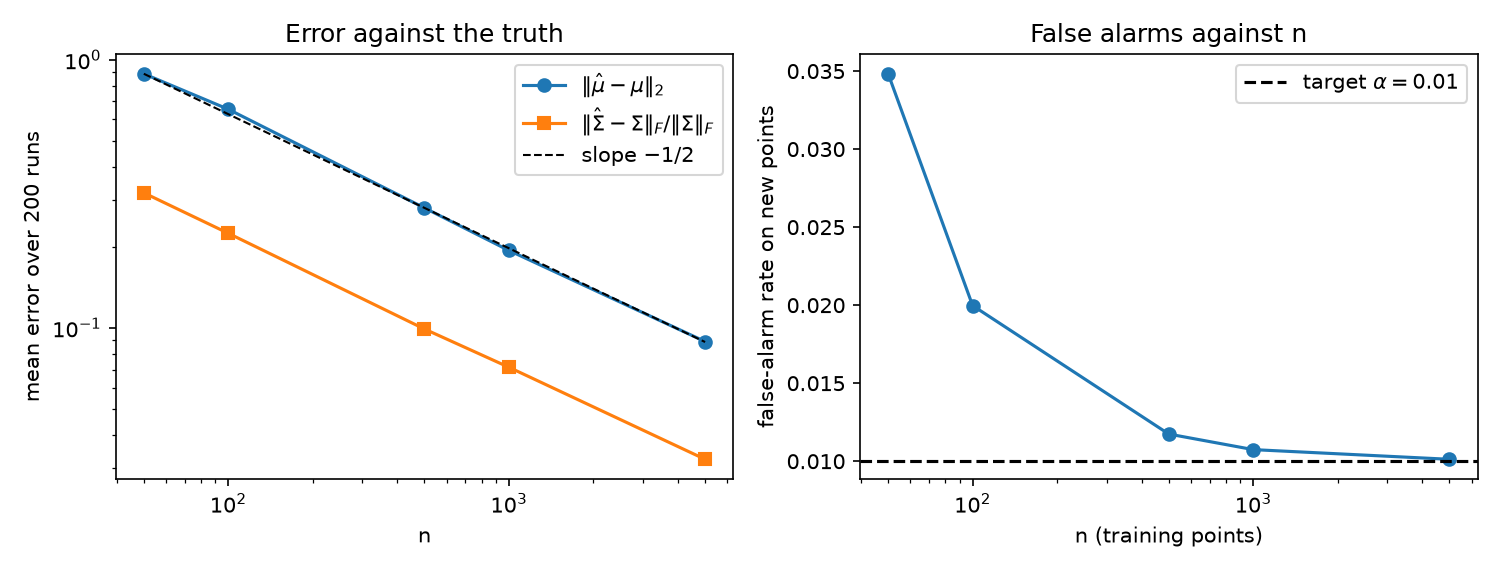
\includegraphics[width=\linewidth]{it3_sim_error_vs_n.png}
\caption{Left: mean error against the truth over 200 runs (log-log axes). Right:
false-alarm rate on new points against the training size $n$.}\label{fig:errn}
\end{figure}

\textbf{Against libraries.} All differences are at rounding level (Table~\ref{tab:verify}).

\textbf{Stress test A: heavy tails (breaks A2).} With multivariate $t$ data (3 degrees of
freedom, same $\mu$ and $\Sigma$), the false-alarm rate is $0.053$ against $\alpha=0.01$,
and $0.0529\pm0.0048$ over 200 runs. The QQ plot bends away from the line
(Figure~\ref{fig:simqq}).

\textbf{Stress test B: a copied feature (breaks A3).} Adding a sixth column equal to
the first makes $\hSigma$ singular (rank 5 of 6). \code{my\_cholesky} stops at pivot 6
(value $-2.7\times10^{-15}$, rounding noise around 0), and \code{numpy.linalg.cond} gives
$7.5\times10^{15}$.

\begin{figure}[H]
\centering
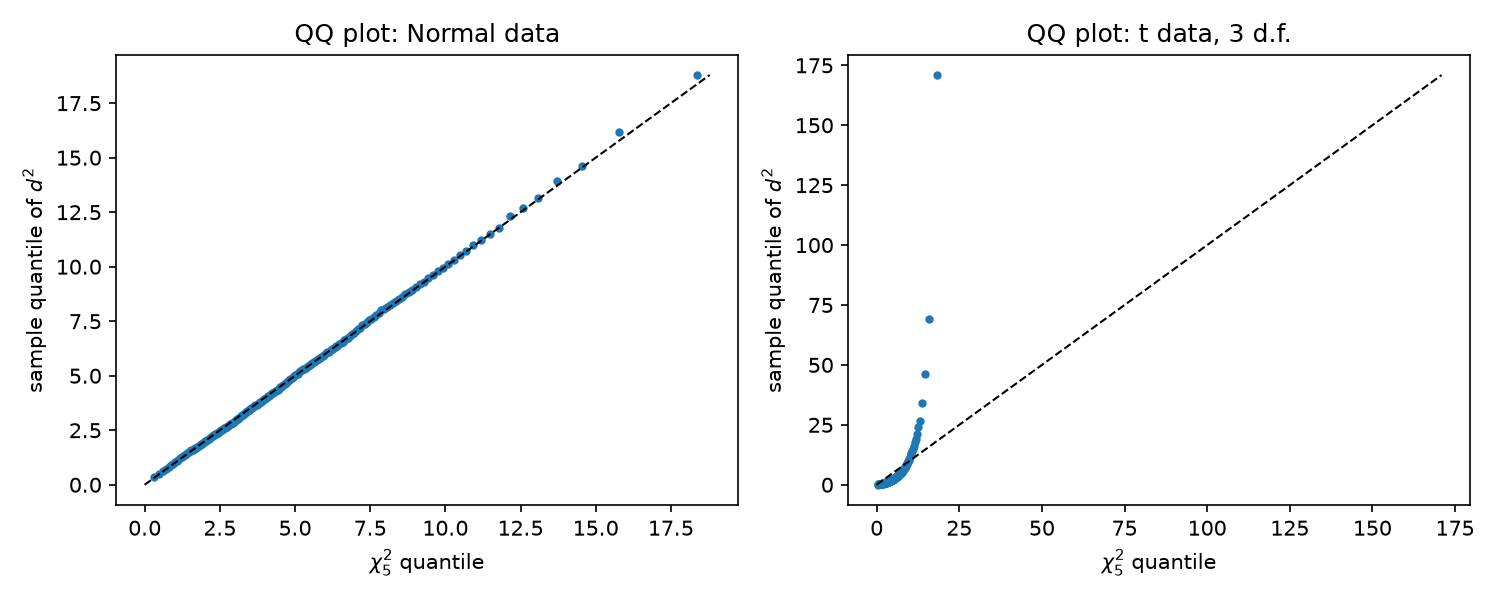
\includegraphics[width=0.9\linewidth]{it3_sim_qq.png}
\caption{QQ plots of $d^2$ against $\chi^2_5$ on simulated data: normal data (left) lie on
the line; $t$ data (right) do not.}\label{fig:simqq}
\end{figure}

% =====================================================================
\section{Real Data}\label{sec:real}

\textbf{Cleaning steps.}
\begin{enumerate}[nosep]
\item Loaded 20,400 rows and 34 columns. Missing values: 0. Duplicate
  (subject, session, repetition) rows: 0. Rows removed: 0.
\item Sorted by subject, session and repetition, and set $r=50(\text{session}-1)+\text{rep}$.
\item Kept the 11 H and 10 UD columns and dropped the 10 DD columns
  ($\text{DD}=\text{H}+\text{UD}$ exactly).
\item Second version: replaced each hold time by its log. All hold times are positive
  (smallest $0.0014$ s); 22,118 UD values are negative, so UD is not logged.
\item Split for the genuine subject s002: training $r=1,\dots,200$ (sessions 1 to 4,
  200 attempts), test $r=201,\dots,400$ (sessions 5 to 8, 200 attempts). Impostors:
  $r=1,\dots,50$ of each of the other 50 subjects (2,500 attempts).
\end{enumerate}

\textbf{Results for s002} ($p=21$, so $\tau=38.93$ at $\alpha=0.01$ and $32.67$ at $\alpha=0.05$):

\begin{table}[H]
\centering\small
\begin{tabular}{@{}llrrr@{}}
\toprule
Features & $\alpha$ & false-alarm rate (test) & detection rate & false-alarm rate (training)\\
\midrule
raw & 0.01 & 0.340 & 0.875 & 0.130\\
raw & 0.05 & 0.390 & 0.926 & 0.170\\
log H & 0.01 & 0.350 & 0.900 & 0.125\\
log H & 0.05 & 0.405 & 0.942 & 0.160\\
\bottomrule
\end{tabular}
\end{table}

\textbf{Every subject as the genuine user} (same protocol, 51 runs):

\begin{table}[H]
\centering\small
\begin{tabular}{@{}llrr@{}}
\toprule
Features & $\alpha$ & mean (median) false-alarm rate & mean (median) detection rate\\
\midrule
raw & 0.01 & 0.173 (0.150) & 0.862 (0.881)\\
raw & 0.05 & 0.236 (0.215) & 0.912 (0.936)\\
log H & 0.01 & 0.145 (0.130) & 0.868 (0.912)\\
log H & 0.05 & 0.195 (0.180) & 0.914 (0.954)\\
\bottomrule
\end{tabular}
\end{table}

\textbf{What this means.} The detector catches most impostors (about 90\%), but it
rejects the genuine user far more often than $\alpha$ promises (about 14\% instead of
1\%). The log transform helps a little on both counts. The main causes are the
heavy-tailed UD features (Question 4) and changes in typing over time
(assumption A5 below). For s002, the test false-alarm rate is driven by session 8,
where every hold time is 3 to 4 standard deviations longer than in training.

\textbf{Library comparison.} Our $\hSigma$, $L$, $\hat d^2$, $\hSigma^{-1}$, $\kappa$ and
$\tau$ agree with NumPy and SciPy to rounding level (Table~\ref{tab:verify}). The
largest absolute difference in $\hat d^2$ is $8.7\times10^{-11}$, but the relative
difference is $6\times10^{-16}$: some impostor attempts have $\hat d^2$ in the tens of
thousands, and rounding error grows with the size of the number.

% =====================================================================
\section{Assumption Checks}\label{sec:assump}
Each check is run first on the simulated data, where the assumption holds by
construction, and then on the real data (s002, log hold times).

\begin{table}[H]
\centering\small
\begin{tabularx}{\linewidth}{@{}l>{\raggedright\arraybackslash}X>{\raggedright\arraybackslash}X>{\raggedright\arraybackslash}p{1.3cm}@{}}
\toprule
 & Simulated data & Real data (s002, log H) & Holds on real data?\\
\midrule
A1 i.i.d. & largest lag-1 autocorrelation of a feature $0.034$, below $3/\sqrt n=0.042$ &
lag-1 autocorrelation of $\hat d^2$ is $0.18$; of the features, median $0.24$ and max
$0.59$, above $3/\sqrt n=0.21$. Mean $\hat d^2$ is $31.0$ in session 1 and $16$ to $20$
in sessions 2 to 4 (the user is still learning) & No\\
A2 normal & $|g_1|\le0.042$, $|g_2|\le0.150$, both within 3 standard errors; KS
$p=0.466$ & 11 of 21 features non-normal (Q4); KS $p<10^{-24}$; false-alarm rate
$0.350$ against $0.01$ & No\\
A3 PD & Cholesky succeeds, $\kappa=2.6$ & Cholesky succeeds, $\kappa=134$ with 21
features; fails with all 31 (Q5) & Yes, after dropping DD\\
A4 $n\gg p$ & $n/p=1000$ & $n/p=9.5$; false-alarm rate $0.90$, $0.53$, $0.35$ when fitting
on the first 50, 100, 200 attempts & Partly\\
A5 stable & fit on the first half, false-alarm rate $0.0112$ on the second half &
false-alarm rate in test sessions 5 to 8: $0.18$, $0.08$, $0.14$, $1.00$ & No\\
A6 impostors differ & detection $0.6028$ on $20{,}000$ attacks, theory $0.6036$ &
detection per impostor: median $1.00$, minimum $0.42$; 2 of 50 impostors detected less
than half the time & Mostly\\
\bottomrule
\end{tabularx}
\end{table}

The simulation shows what passing looks like, and the code is correct. On the real
data, A1, A2 and A5 fail, so the $\chi^2$ threshold does not give the promised
false-alarm rate. This is a property of the data, not of the code.

% =====================================================================
\section{Verification Table}
\begin{table}[H]
\centering\small
\begin{tabular}{@{}lllll@{}}
\toprule
Data & Quantity & Compared with & Difference & Pass?\\
\midrule
Small example & $d^2$ & exact fraction ($4$) & $4.0\times10^{-15}$ & $\checkmark$\\
Small example & $\hSigma\hSigma^{-1}$ & $I$ & $0$ (exact) & $\checkmark$\\
Small example & $\tau$ ($p=2$) & $-2\log\alpha$ & $1.3\times10^{-13}$ & $\checkmark$\\
Simulation ($n=5000$) & $\hmu$ & true $\mu$ & max $1.56$ SE & $\checkmark$\\
Simulation ($n=5000$) & $\hSigma$ & true $\Sigma$ & max $1.99$ SE & $\checkmark$\\
Simulation ($n=50$ to $5000$) & error slope & $-1/2$ & $-0.505$, $-0.497$ & $\checkmark$\\
Simulation ($n=5000$) & false-alarm rate & $\alpha=0.01$ & $0.0102\in[0.0058,0.0142]$ & $\checkmark$\\
Simulation ($n=5000$) & $\hSigma$ & \code{np.cov(bias=True)} & max $|\cdot|=1.8\times10^{-15}$ & $\checkmark$\\
Simulation ($n=5000$) & $L$ & \code{np.linalg.cholesky} & max $|\cdot|=8.7\times10^{-19}$ & $\checkmark$\\
Simulation ($n=5000$) & $d^2$ & \code{np.linalg.inv} & max $|\cdot|=7.1\times10^{-15}$ & $\checkmark$\\
Simulation ($n=5000$) & $\hSigma^{-1}$ & \code{np.linalg.inv} & max $|\cdot|=2.8\times10^{-17}$ & $\checkmark$\\
Simulation ($n=5000$) & $\tau$ & \code{scipy.stats.chi2} & max $|\cdot|=2.5\times10^{-13}$ & $\checkmark$\\
Simulation ($n=5000$) & $\kappa(\hSigma)$ & \code{np.linalg.cond} & rel.\ $1.4\times10^{-13}$ & $\checkmark$\\
Simulation (stress A, $t$) & false-alarm rate & $\alpha=0.01$ & $0.053$ (5 times too high) & $\checkmark$ (as expected)\\
Simulation (stress B, copy) & Cholesky & & stops at pivot 6 & $\checkmark$ (as expected)\\
Real data (log H) & $\hSigma$ & \code{np.cov(bias=True)} & max $|\cdot|=1.4\times10^{-17}$ & $\checkmark$\\
Real data (log H) & $L$ & \code{np.linalg.cholesky} & max $|\cdot|=2.8\times10^{-17}$ & $\checkmark$\\
Real data (log H) & $\hat d^2$ & \code{np.linalg.inv} & rel.\ $6.2\times10^{-16}$ & $\checkmark$\\
Real data (log H) & $\hSigma^{-1}$ & \code{np.linalg.inv} & rel.\ $5.1\times10^{-16}$ & $\checkmark$\\
Real data (log H) & $\kappa(\hSigma)$ & \code{np.linalg.cond} & rel.\ $6.4\times10^{-16}$ & $\checkmark$\\
Real data & $\tau$ ($p=21$) & \code{scipy.stats.chi2} & max $|\cdot|=1.5\times10^{-12}$ & $\checkmark$\\
\bottomrule
\end{tabular}
\caption{Verification table. Every number is printed by \code{small\_example.py},
\code{check\_simulation.py} or \code{run\_real.py}.}\label{tab:verify}
\end{table}

\bigskip
\textbf{Reference.} K.~S.~Killourhy and R.~A.~Maxion, \emph{Comparing
anomaly-detection algorithms for keystroke dynamics}, IEEE/IFIP International
Conference on Dependable Systems and Networks (DSN), 2009.

\end{document}
